
\documentclass{article}
\usepackage[utf8]{inputenc}
\usepackage{graphicx}
\usepackage{listings}
\usepackage{xcolor}
\usepackage{float}  % Add float package to control figure placement
\usepackage{amsmath}

\title{09a ZRX543 4x4 Keypad Introduction}
\author{Nicholas Bruzzese}
\date{\today}

\definecolor{dkgreen}{rgb}{0,0.6,0}
\definecolor{gray}{rgb}{0.5,0.5,0.5}
\definecolor{mauve}{rgb}{0.58,0,0.82}

\lstset{frame=tb,
	language=Python,
	aboveskip=3mm,
	belowskip=3mm,
	showstringspaces=false,
	columns=flexible,
	basicstyle={\small\ttfamily},
	numbers=none,
	numberstyle=\tiny\color{gray},
	keywordstyle=\color{blue},
	commentstyle=\color{dkgreen},
	stringstyle=\color{mauve},
	breaklines=true,
	breakatwhitespace=true,
	tabsize=3
}

\begin{document}
	
	\maketitle
	
	\section*{What is a 4x4 Keypad?}
	The ZRX543 4x4 keypad is a matrix-style keypad with 16 buttons arranged in a 4x4 grid. It uses a combination of rows and columns to detect button presses. Each button connects one row to one column, enabling the identification of the pressed button.
	
	\subsection*{Key Features}
	\begin{itemize}
		\item \textbf{Compact Design}: 16 keys arranged in a small footprint.
		\item \textbf{Matrix Configuration}: Reduces the number of GPIO pins required.
		\item \textbf{Versatility}: Commonly used in security systems, robotics, and more.
	\end{itemize}
	
	\section*{Hardware Requirements}
	\begin{itemize}
		\item Raspberry Pi (any model with GPIO pins).
		\item ZRX543 4x4 keypad.
		\item Jumper wires for connections.
	\end{itemize}
	
	\section*{Wiring Diagram}
	\begin{figure}[H]
		\centering
		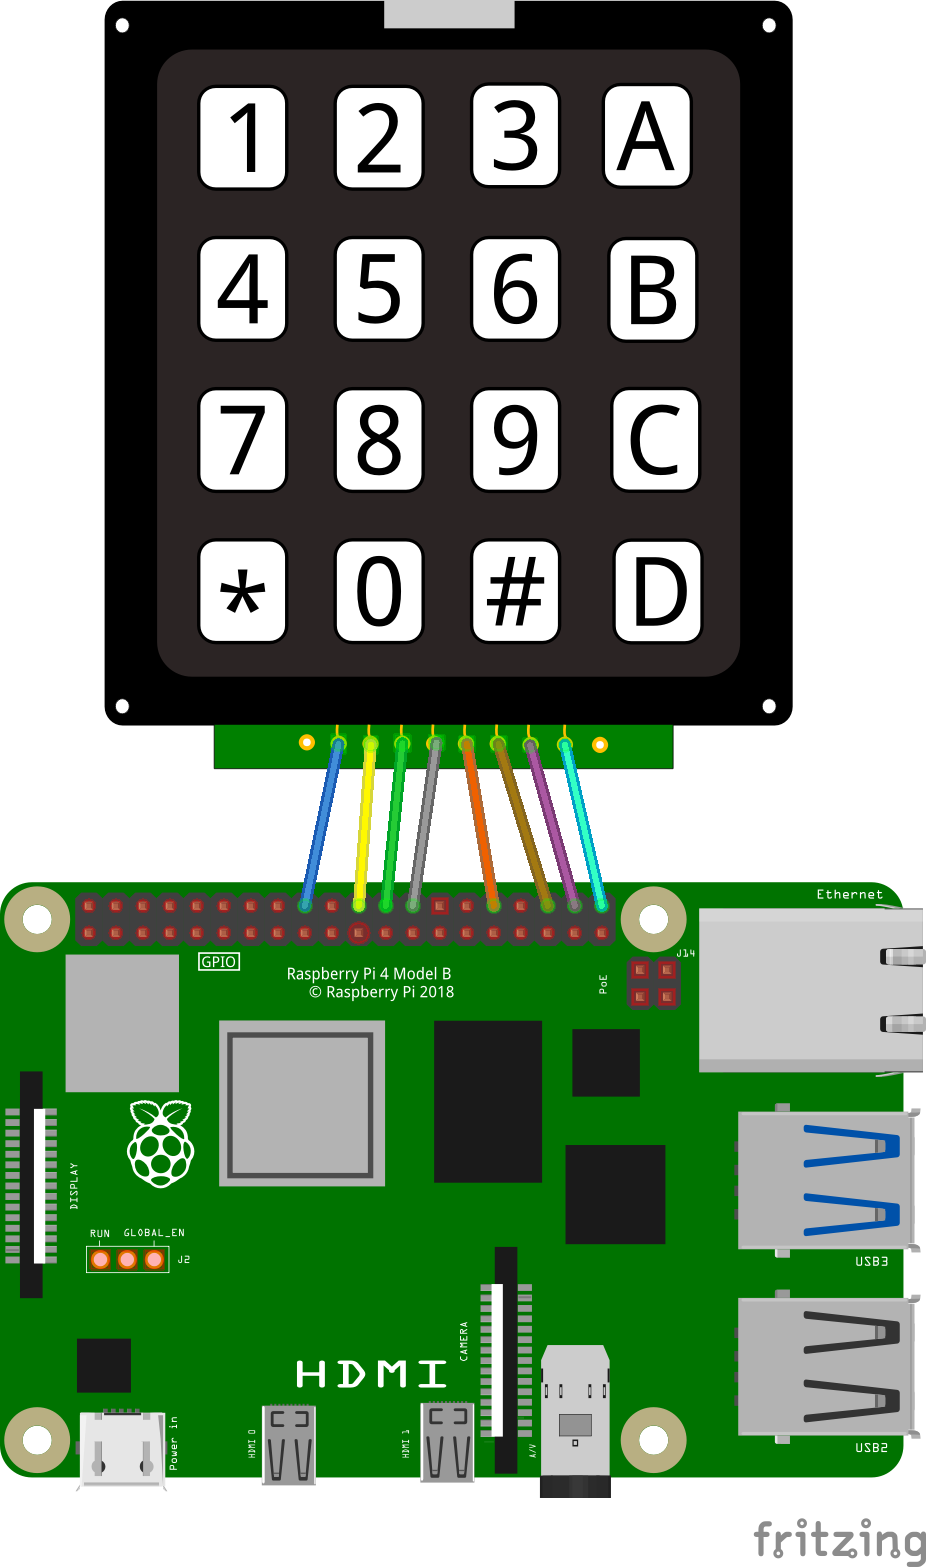
\includegraphics[width=0.8\textwidth]{09a-keypad-intro-diagram.png} % Adjust width to 80% of text width
		\caption{Wiring Diagram}
	\end{figure}
	
	\section*{Connections}
	
	The ZRX543 4x4 keypad has 8 pins: 4 rows (R1 to R4) and 4 columns (C1 to C4). These need to be connected to the GPIO pins of the Raspberry Pi. The connections are as follows:
	
	\begin{center}
		\begin{tabular}{|l|l|}
			\hline
			\textbf{Keypad Pin} & \textbf{GPIO Pin} \\
			\hline
			R1 (A8)    & GPIO 24  \\
			R2 (A7)    & GPIO 25  \\
			R3 (A6)    & GPIO 8   \\
			R4 (A5)    & GPIO 7   \\
			C1 (A4)    & GPIO 12  \\
			C2 (A3)    & GPIO 16  \\
			C3 (A2)    & GPIO 20  \\
			C4 (A1)    & GPIO 21  \\
			\hline
		\end{tabular}
	\end{center}
	
	Ensure the keypad is connected securely, and double-check the pin mappings before proceeding.
	
	\section*{Code Explanation}
	
	The Python script below scans the keypad, detects button presses, and prints the corresponding key.
	
	\subsection*{1. GPIO Initialization}
	The rows are configured as output pins, and the columns are configured as input pins with internal pull-down resistors to detect button presses.
	
	\begin{lstlisting}
		import RPi.GPIO as GPIO
		import time
		
		# GPIO pin definitions
		L1 = 24  # Row 1
		L2 = 25  # Row 2
		L3 = 8   # Row 3
		L4 = 7   # Row 4
		C1 = 12  # Column 1
		C2 = 16  # Column 2
		C3 = 20  # Column 3
		C4 = 21  # Column 4
		
		# GPIO setup
		GPIO.setwarnings(False)
		GPIO.setmode(GPIO.BCM)
		GPIO.setup([L1, L2, L3, L4], GPIO.OUT)
		GPIO.setup([C1, C2, C3, C4], GPIO.IN, pull_up_down=GPIO.PUD_DOWN)
	\end{lstlisting}
	
	\subsection*{2. Scanning the Keypad}
	The \texttt{readLine} function activates one row at a time and checks all columns for a signal. If a signal is detected, the corresponding key is printed.
	
	\begin{lstlisting}
		def readLine(line, characters):
		GPIO.output(line, GPIO.HIGH)
		if GPIO.input(C1) == 1:
		print(characters[0])
		if GPIO.input(C2) == 1:
		print(characters[1])
		if GPIO.input(C3) == 1:
		print(characters[2])
		if GPIO.input(C4) == 1:
		print(characters[3])
		GPIO.output(line, GPIO.LOW)
	\end{lstlisting}
	
	\subsection*{3. Main Loop}
	The main loop continuously scans the keypad by calling \texttt{readLine} for each row. The detected key is printed to the console.
	
	\begin{lstlisting}
		try:
		while True:
		readLine(L1, ["1", "2", "3", "A"])
		readLine(L2, ["4", "5", "6", "B"])
		readLine(L3, ["7", "8", "9", "C"])
		readLine(L4, ["*", "0", "#", "D"])
		time.sleep(0.1)
		except KeyboardInterrupt:
		print("\nApplication stopped!")
	\end{lstlisting}
	
	\section*{Running the Project}
	
	\begin{enumerate}
		\item Save the code as \texttt{keypad.py}.
		\item Run the script:
		\begin{lstlisting}
			python3 keypad.py
		\end{lstlisting}
		\item Press buttons on the keypad. The corresponding key will be printed in the terminal.
	\end{enumerate}
	
	\section*{Experiment Ideas}
	\begin{itemize}
		\item \textbf{Key Combination Detection}: Add logic to detect specific key sequences, such as a password.
		\item \textbf{Interactive Menus}: Combine the keypad with an LCD to create a basic user interface.
		\item \textbf{Custom Actions}: Trigger GPIO actions (e.g., turning on an LED) based on specific keys.
	\end{itemize}
	
	\section*{Applications}
	\begin{itemize}
		\item Security systems (e.g., digital locks).
		\item Menu-driven systems for user interaction.
		\item Custom input devices for Raspberry Pi projects.
	\end{itemize}
	
	With this project, you've built a solid foundation for using keypads with Raspberry Pi. Want to take it further? Try integrating the keypad into a more complex system like a smart home controller or a robotics interface!
	
\end{document}
